\documentclass[conference]{IEEEtran}

\usepackage{amsmath,amssymb,amsfonts,amsthm,booktabs,graphicx}
\usepackage{url}
\interdisplaylinepenalty=2500
\DeclareMathOperator*{\argmax}{arg\,max}

\newtheorem{theorem}{Theorem}
\newtheorem{proposition}[theorem]{Proposition}
\newtheorem{lemma}[theorem]{Lemma}
\newtheorem{corollary}[theorem]{Corollary}
\newtheorem{definition}[theorem]{Definition}
\newtheorem{example}[theorem]{Example}
\newtheorem{remark}[theorem]{Remark}

\newcommand{\Z}{\mathbb{Z}}
\newcommand{\E}{\mathbb{E}}
\newcommand{\Prob}{\mathbb{P}}
\newcommand{\ccrit}{c_{\mathrm{crit}}}

\begin{document}

\title{Optimal Additive Integer Masks for One-Guess Vulnerability under an Absolute-Moment Budget}

\author{
\IEEEauthorblockN{Anonymous Author(s)}
\IEEEauthorblockA{Anonymous Institution}
}

\maketitle

\begin{abstract}
We study the average one-guess success probability of an adversary who observes the ordinary integer sum of a finite-support secret and an independent integer-valued mask, subject to an absolute-moment budget on the mask. For a uniform secret on an interval the exact optimum and an explicit optimiser are obtained. For a biased bit the masks that achieve no increase over the prior baseline are characterised, and the entire cost--vulnerability frontier is determined. It is the piecewise-linear interpolation of an explicit sequence of points generated by cost-optimally shifted truncated geometric masks. It has infinitely many affine pieces, which accumulate at the critical cost, where the frontier meets the prior baseline with zero slope. The proof rests on a layer-cake decomposition of an arbitrary mask into truncated geometrics, along which both the vulnerability and the cost are exactly additive. The results give exact design guidance for additive integer noise under the average one-guess metric.
\end{abstract}

\begin{IEEEkeywords}
Bayes vulnerability, quantitative information flow, additive noise, absolute-moment constraint, geometric distributions
\end{IEEEkeywords}

\section{Introduction}
Quantitative information flow measures how much an observation helps an adversary guess a secret. The most basic operational criterion is the probability that the adversary's single best guess is correct. This is the Bayes vulnerability \(V(X)=\max_x\Prob(X=x)\) before the observation and the posterior vulnerability
\[
V(X\mid Y)=\sum_y\max_x\Prob(X=x,Y=y)
\]
after observing \(Y\)~\cite{Smith09}. Minimising \(V(X\mid Y)\) is therefore equivalent to maximising average conditional min-entropy. In privacy-enhancing technologies this quantity is a direct measure of the residual risk that a one-guess adversary can still recover the secret after noise has been added.

We consider the additive channel
\[
Y=X+N
\]
in which an independent integer-valued mask \(N\) is added to a finite-support integer-valued secret \(X\). The design question is how to choose the law \(q\) of \(N\) so as to minimise average one-guess success subject to an absolute-moment budget \(\E|N|\le c\). Absolute-moment costs arise naturally when the practical price of noise is proportional to its magnitude. The goal is exact design guidance: the minimal vulnerability achievable under a given budget, and an explicit mask that attains it.

\subsection{Contributions}
\begin{enumerate}
\item For a uniform secret on an interval of length \(m\) the exact minimal vulnerability and an explicit optimiser are determined (Theorem~\ref{thm:uniform}).
\item For a biased bit all masks that produce no extra average guessing advantage are characterised, the exact critical cost and the strict gap below it are given, and the exact initial segment is determined (Theorems~\ref{thm:zero}--\ref{thm:initial}).
\item For every bias \(p\in(1/2,1)\) the complete frontier is determined (Theorem~\ref{thm:frontier}). It is the linear interpolation of explicit points \(Q_k\), \(k\ge1\), obtained from truncated geometric masks of length \(k\), and it has infinitely many affine pieces accumulating at the critical cost (Corollary~\ref{cor:pieces}). On every piece an optimiser is a mixture of two adjacent truncated geometrics, with a free residual at exactly one endpoint (Corollary~\ref{cor:structure}). The first two pieces beyond the initial segment can also be certified directly by dual multipliers (Corollary~\ref{cor:cells}). Figure~\ref{fig:frontier} shows the frontier.
\end{enumerate}

\section{Related work}
Smith~\cite{Smith09} introduced Bayes vulnerability and min-entropy leakage. Dodis, Ostrovsky, Reyzin and Smith~\cite{DORS08} defined average min-entropy. Braun, Chatzikokolakis and Palamidessi~\cite{BCP09} compared additive and multiplicative one-try leakage. Issa, Wagner and Kamath~\cite{IWK20} showed that maximal leakage for finite alphabets equals \(\log\sum_y\max_{x:p(x)>0}\Prob(Y=y\mid X=x)\). Maximal leakage therefore also admits an operational interpretation as the log of the average one-guess advantage under the worst-case prior. Under an absolute-moment budget on additive integer noise, however, the mechanism that minimises maximal leakage is not the same as the mechanism that minimises Bayes vulnerability for a fixed prior. In particular, the truncated-geometric masks that achieve the frontier derived in this paper are optimal for the prior-specific one-guess metric, but they are not in general optimal for maximal leakage. Conversely, a maximal-leakage optimal mechanism under the same cost can leave a given biased bit more vulnerable than the frontier \(V_p^*(c)\). The two metrics therefore supply different design guidance even when the cost constraint is identical.

Saeidian, Cervia, Oechtering and Skoglund~\cite{SCOS21} solved a privacy--utility problem under maximal leakage and expected Hamming distortion; the mechanisms here are restricted to be additive and the cost is an absolute moment. Asoodeh et al.~\cite{Asoodeh17} studied privacy-constrained guessing probabilities under a different formulation that does not specialise to additive integer masks with an absolute-moment budget. Geng, Ding, Guo and Kumar~\cite{GDGK19} derived optimal additive noise for differential privacy under \(\ell_1\) and \(\ell_2\) costs; the constraint is differential privacy, not Bayes vulnerability.

Side-channel masking literature (e.g., the noisy-leakage model of Prouff and Rivain~\cite{PR13}) addresses a different threat model based on shares. A targeted search of the primary quantitative-information-flow, maximal-leakage, differential-privacy-noise, and guessing-with-noise literature did not locate prior solutions of the exact cost-constrained additive-integer problems studied here.

\section{Preliminaries}
Let \(X\) have finite support and law \(p\), and let \(N\) be independent with law \(q\) on \(\Z\). Set \(Y=X+N\).

\begin{proposition}[MAP rule]\label{prop:map}
The optimal one-guess success probability is
\[
V(X\mid Y)=\sum_{y\in\Z}\max_x p(x)q(y-x),
\]
attained by any \(g(y)\in\argmax_x p(x)q(y-x)\). In particular \(V(X\mid Y)\ge V(X)\).
\end{proposition}
\begin{proof}
A strategy \(g\) succeeds with probability \(\sum_y p(g(y))q(y-g(y))\); maximise each term separately. For any fixed \(x_0\), the sum is at least \(p(x_0)\).
\end{proof}

For a fixed secret distribution the optimisation is over all probability laws \(q\) on \(\Z\) with \(\E_q|N|\le c\). The optimal value is denoted \(V^*(c)\).

\section{Uniform interval secret}
Let \(X\) be uniform on \(I_m=\{0,\dots,m-1\}\). Then
\[
V(q)=\frac1m\sum_y\max_{x\in I_m}q(y-x).
\]

\begin{lemma}[Layer cake]\label{lem:layer}
Let \(h=\|q\|_\infty\) and \(B_t=\{y:q(y)>t\}\). Then \(mV(q)=\int_0^h|B_t+I_m|\,dt\).
\end{lemma}
\begin{proof}
For each \(s\), \(\max_{y\in s-I_m}q(y)=\int_0^h\mathbf 1[y\in B_t+I_m]\,dt\). Sum over \(s\) and apply Tonelli's theorem.
\end{proof}

\begin{lemma}[One-dimensional sumset]\label{lem:sumset}
For nonempty finite \(A\subset\Z\), \(|A+I_m|\ge|A|+m-1\). For \(m\ge2\), equality holds if and only if \(A\) is an interval of integers.
\end{lemma}
\begin{proof}
\(A+I_m\supseteq A\cup(\max A+I_m)\), and the two sets meet only in \(\max A\). If \(A\) is an interval the sumset is an interval of the stated cardinality. If consecutive elements of \(A\) differ by at least \(2\), a gap point appears in the sumset.
\end{proof}

\begin{lemma}[Cheapest mask of given peak]\label{lem:fill}
For \(h\in(0,1]\) let \(r\ge0\) satisfy \(1/(2r+3)<h\le1/(2r+1)\) and \(\rho=1-(2r+1)h\in[0,2h)\). Let \(q_h\) place mass \(h\) on each of \(\{-r,\dots,r\}\) and \(\rho/2\) on each of \(\pm(r+1)\). Then \(\E_q|N|\ge C(h):=\E_{q_h}|N|=(r+1)(1-(r+1)h)\) for every \(q\) with \(\|q\|_\infty\le h\).
\end{lemma}
\begin{proof}
Direct computation gives the cost formula. Let \(R=r+1\) and \(\Delta=q-q_h\). For \(|y|<R\) both factors \(|y|-R\le0\) and \(\Delta(y)\le0\), so their product is nonnegative. For \(|y|=R\) the term vanishes. For \(|y|>R\) both factors are nonnegative. Hence \(\sum(|y|-R)\Delta(y)\ge0\).
\end{proof}

\begin{theorem}[Uniform secret]\label{thm:uniform}
Let \(r\ge0\) satisfy \(r(r+1)/(2r+1)\le c\le(r+1)(r+2)/(2r+3)\). Set \(h^*(c)=(r+1-c)/(r+1)^2\). Then
\[
\min_{\E|N|\le c}V(q)=\frac{1+(m-1)h^*(c)}{m},
\]
attained by \(q_{h^*(c)}\).
\end{theorem}
\begin{proof}
Lemmas~\ref{lem:layer} and~\ref{lem:sumset} together with \(\int_0^h|B_t|\,dt=1\) give \(mV(q)\ge1+(m-1)\|q\|_\infty\). The cost constraint and Lemma~\ref{lem:fill} force \(\|q\|_\infty\ge h^*(c)\). The candidate has cost exactly \(c\) and interval superlevel sets, so equality holds throughout. The argument covers infinite-support competitors. For \(m=1\) or \(c=0\) one has \(V\equiv1\).
\end{proof}

The optimiser is not in general uniform on an interval. Asymptotically, the cost of a height-\(h\) filled peak is \(C(h)\sim1/(4h)\) (the continuous water-filling limit), so \(h^*(c)\sim1/(4c)\).

\section{Biased bit}
Let \(\Prob(X=0)=p\in(1/2,1)\), \(\Prob(X=1)=1-p\), and \(a=(1-p)/p\in(0,1)\). Define
\[
V_p(q)=\sum_y\max\bigl\{p\,q(y),(1-p)q(y-1)\bigr\}
\]
and
\[
V_p^*(c)=\inf\{V_p(q):\E_q|N|\le c\}.
\]
The baseline is \(V(X)=p\). Equivalently,
\[
V_p(q)=p+\sum_y\max\bigl(0,(1-p)q(y-1)-p\,q(y)\bigr).
\]
For \(p=1/2\) the problem is the case \(m=2\) of Theorem~\ref{thm:uniform}.

\begin{theorem}[Zero extra average advantage]\label{thm:zero}
\(V_p(q)=p\) if and only if \(q(n)\ge a\,q(n-1)\) for every \(n\in\Z\). Such laws are precisely the mixtures \(q=\sum_L w_L G_L\), where \(G_L(n)=(1-a)a^{n-L}\mathbf 1_{n\ge L}\), \(w_L\ge0\) and \(\sum_L w_L=1\).
\end{theorem}
\begin{proof}
The first claim is immediate from the excess representation. Given the inequality, set \(d(n)=q(n)-a\,q(n-1)\ge0\). Iterating and using \(a^k q(n-k)\to0\) yields \(q(n)=\sum_{L\le n}d(L)a^{n-L}\). Summing over \(n\) gives \(\sum d(L)=1-a\), so the weights \(w_L=d(L)/(1-a)\) produce the claimed mixture. Conversely each \(G_L\) satisfies the inequality, which is preserved by mixtures.
\end{proof}

\begin{corollary}
No finite-support mask achieves \(V_p(q)=p\). If \(q(n_0)>0\) then the ratio inequality forces \(q(n_0+k)\ge a^k q(n_0)>0\) for all \(k\ge0\).
\end{corollary}

\begin{remark}
\(V_p(q)=p\) concerns the average only. For a pure geometric the posterior at the left endpoint equals \(1\), and \(Y\) is never independent of \(X\).
\end{remark}

\begin{theorem}[Critical cost]\label{thm:ccrit}
\[
c_{\mathrm{crit}}(p)=\min_{\ell\in\Z_{\ge0}}\Bigl(\ell+\frac{a(2a^\ell-1)}{1-a}\Bigr),
\]
attained at \(\ell^*=\#\{j\ge1:a^j>1/2\}=\lceil\log2/\log(1/a)\rceil-1\) (an integer median; with a tie when \(a^{\ell^*+1}=1/2\)). Moreover \(V_p^*(c)=p\) for \(c\ge c_{\mathrm{crit}}(p)\) and \(V_p^*(c)>p\) for \(c<c_{\mathrm{crit}}(p)\).
\end{theorem}
\begin{proof}
By Theorem~\ref{thm:zero} and linearity the cost of a zero-advantage mask is at least the minimum over pure shifts. For positive shifts the cost is larger, so it suffices to minimise \(f(\ell)=\E|G-\ell|\) over \(\ell\ge0\). The difference \(f(\ell+1)-f(\ell)=1-2a^{\ell+1}\) changes sign at the stated integer, with a tie exactly when equality holds.

Existence of minimisers: a minimising sequence with \(\E|N|\le c\) is tight by Markov's inequality. A diagonal argument yields a subsequence converging pointwise to some \(q\). Tightness implies \(\sum q=1\). Fatou's lemma gives \(\E_q|N|\le c\). Scheff\'e's lemma then upgrades the convergence to \(\ell^1\). The bound \(|V_p(q)-V_p(q')|\le\|q-q'\|_1\) gives continuity of the objective, so a minimiser exists. (The case \(c=0\) is covered by Theorem~\ref{thm:initial}.) If \(V_p^*(c)=p\) for some \(c<c_{\mathrm{crit}}(p)\), the minimiser would be a zero-advantage mask of cost strictly below \(c_{\mathrm{crit}}(p)\), a contradiction. For \(c\ge c_{\mathrm{crit}}(p)\) the geometric at the optimal shift is feasible.
\end{proof}

\begin{theorem}[Initial segment]\label{thm:initial}
For \(0\le c\le1-p\), \(V_p^*(c)=1-pc\), attained by \(q=(1-c)\delta_0+c\delta_1\). Moreover \(V_p(q)\ge1-p\,\E|N|\) for every \(q\).
\end{theorem}
\begin{proof}
Choosing the first term of the maximum for \(s\le0\) and the second for \(s\ge1\),
\begin{align*}
V_p(q)&\ge p\Pr(N\le0)+(1-p)\Pr(N\ge0)\\
&=1-p\Pr(N>0)-(1-p)\Pr(N<0)\\
&\ge1-p\Pr(N\ne0)\ge1-p\,\E|N|,
\end{align*}
using \(1-p<p\) and \(\mathbf 1[y\ne0]\le|y|\) on \(\Z\). The two-point mask has cost \(c\) and vulnerability \(1-pc\) on the stated interval.
\end{proof}

\subsection{Layer-cake decomposition into truncated geometrics}
The key technical tool is an explicit layer-cake representation that decomposes an arbitrary mask \(q\) into a mixture of truncated geometric components, with exact additivity of both vulnerability and cost.

Define the excess process relative to the geometric ratio \(a\). For a law \(q\), set
\[
d(n)=q(n)-a\,q(n-1),\qquad s\in\Z.
\]
Note that \(\sum_n d(n)=(1-a)\) whenever \(\sum q=1\) and the boundary terms vanish (which they do under the absolute-moment constraint). The positive parts of the excesses can be layered as follows.

\textbf{Peeling construction.} Initialise the residual measure \(q^{(0)}=q\). At stage \(i=0,1,2,\dots\), while the residual \(q^{(i)}\) is not identically zero, let
\[
L_i=\min\{s:q^{(i)}(s)>0\}
\]
be the leftmost point of positive mass (finite almost surely under \(\E|N|<\infty\)). Define the maximal length \(k_i\in\{1,2,\dots,\infty\}\) such that the residual admits a truncated geometric component of length \(k_i\) starting at \(L_i\):
\[
k_i=\sup\bigl\{k\ge1:\ q^{(i)}(L_i+j)\ge a^j\,q^{(i)}(L_i)\ \text{for all}\ 0\le j<k\bigr\},
\]
with the convention \(k_i=\infty\) if the inequality holds for every finite \(k\). Let \(\alpha_i=q^{(i)}(L_i)/(1-a^{k_i})\) if \(k_i<\infty\), or \(\alpha_i=q^{(i)}(L_i)/(1-a)\) if \(k_i=\infty\). Subtract the scaled truncated geometric
\[
\alpha_i\,T_{L_i,k_i}
\]
from the residual (this is nonnegative by construction of \(k_i\)) to obtain the next residual \(q^{(i+1)}\). The process terminates after finitely many steps almost surely, or produces a countable sum that converges in \(\ell^1\).

The resulting weights \(\alpha_i\) and components \((L_i,k_i)\) define a discrete probability measure \(\nu\) on the space of truncated geometrics (normalised so that \(\sum\alpha_i=1\)) satisfying
\[
q=\sum_i\alpha_i\,T_{L_i,k_i}.
\]
Because each peeled component contributes exactly its own excess to the vulnerability representation and the absolute-moment cost is linear, we obtain the exact additivity
\[
V_p(q)=\sum_i\alpha_i\,V_p(T_{L_i,k_i}),\qquad
\E_q|N|=\sum_i\alpha_i\,\E_{T_{L_i,k_i}}|N|.
\]
(The same identities hold for the continuous mixture representation \(\int T_{L,k}\,d\nu\).)

This decomposition reduces the original infinite-dimensional optimisation to a convex combination of the elementary truncated-geometric problems solved next. The algebraic verification of the peeling invariants and the additivity identities is confirmed by the accompanying exact-arithmetic scripts.

\subsection{The frontier}
\begin{proposition}[Monotonicity and convexity]\label{prop:convex}
The function \(V_p^*\) is nonincreasing and convex on \([0,\infty)\). It is continuous on \((0,\infty)\). Continuity at \(0\) follows from Theorem~\ref{thm:initial}.
\end{proposition}
\begin{proof}
If \(c\le c'\) the feasible set for \(c\) is contained in that for \(c'\), so \(V_p^*\) is nonincreasing. The function \(V_p\) is convex, since a maximum of linear functions is convex and sums of convex functions are convex. For convexity, take feasible masks \(q_0,q_1\) for budgets \(c_0,c_1\) and \(\theta\in[0,1]\). The mixture \(\theta q_0+(1-\theta)q_1\) is feasible for \(\theta c_0+(1-\theta)c_1\) and, by convexity of \(V_p\), has vulnerability at most the corresponding convex combination. Taking infima yields convexity of \(V_p^*\). A finite convex function on an open interval is continuous, so \(V_p^*\) is continuous on \((0,\infty)\).
\end{proof}

\begin{definition}[Truncated geometrics and the points \(Q_k\)]\label{def:Q}
For \(L\in\Z\) and \(k\in\{1,2,\dots\}\) let
\[
T_{L,k}(s)=\frac{1-a}{1-a^k}\,a^{s-L}\,\mathbf 1\{L\le s\le L+k-1\},
\]
and put \(T_{L,\infty}=G_L\). For \(k\ge1\) and \(m\ge0\) write
\[
u_k=\frac{a^k}{1-a^k},\qquad A_m=\sum_{i=1}^m a^i=\frac{a(1-a^m)}{1-a},
\]
\[
m_k=\#\{1\le j\le k-1:\ 2a^j>1+a^k\},
\]
and define
\begin{align*}
V_k&=p+(2p-1)\,u_k,\\
C_k&=\frac{a}{1-a}+(m_k-2A_{m_k})+u_k\bigl(2(m_k-A_{m_k})-k\bigr),
\end{align*}
\(Q_k=(C_k,V_k)\), and \(Q_\infty=(\ccrit(p),p)\). An index \(k\) is a \emph{transition} if \(m_{k+1}=m_k+1\), and a \emph{tie} if \(2a^{m_k+1}=1+a^k\).
\end{definition}

For example \(Q_1=(0,1)\) is the point mass \(\delta_0\) and \(Q_2=(1-p,\,1-p+p^2)\).

\begin{theorem}[Biased-bit frontier]\label{thm:frontier}
Let \(p\in(1/2,1)\). Then \(0=C_1<C_2<C_3<\cdots\), \(C_k\to\ccrit(p)\), \(V_k\downarrow p\), and
\[
V_p^*(c)=\begin{cases}
V_k-\sigma_k\,(c-C_k), & C_k\le c\le C_{k+1},\ k\ge1,\\
p, & c\ge\ccrit(p),
\end{cases}
\]
with slopes
\begin{align*}
\sigma_k&=\frac{V_k-V_{k+1}}{C_{k+1}-C_k}=\frac{2p-1}{E_k},\\
E_k&=k-A_k-2(m_k-A_{m_k})-\theta_k(1-a^k),
\end{align*}
where
\[
\theta_k=\begin{cases}0,& m_{k+1}=m_k,\\[1mm] \dfrac{2a^{m_k+1}-1-a^{k+1}}{a^k(1-a)}\in(0,1],& m_{k+1}=m_k+1.\end{cases}
\]
The slopes satisfy \(\sigma_1\ge\sigma_2\ge\cdots>0\) and \(\sigma_k\to0\), and \(\sigma_{k-1}=\sigma_k\) holds if and only if \(k\) is a tie. For \(C_k\le c\le C_{k+1}\) an optimiser is the mixture
\[
q_c=\vartheta T_{-m_k,k}+(1-\vartheta)T_{-m_{k+1},k+1},\qquad
\vartheta=\frac{C_{k+1}-c}{C_{k+1}-C_k}.
\]
Figure~\ref{fig:frontier} shows the resulting frontier for several values of the bias. Figure~\ref{fig:ccrit} shows how the critical cost depends on the bias. Figure~\ref{fig:optimiser} shows a typical optimal mask on an intermediate piece.

\begin{example}[Numerical illustration]
For \(p=0.7\) one has \(a=3/7\), \(\ell^*=1\), and \(c_{\mathrm{crit}}(0.7)\approx 1.4286\). The first points are
\[
Q_1=(0,1),\quad Q_2\approx(0.3,0.79),\quad Q_3\approx(0.6429,0.7429).
\]
On the piece \([C_2,C_3]\) the optimiser is the mixture of the optimally shifted length-2 and length-3 truncated geometrics with weights linear in \(c\).
\end{example}
\end{theorem}

\begin{figure*}[t!]
\centering
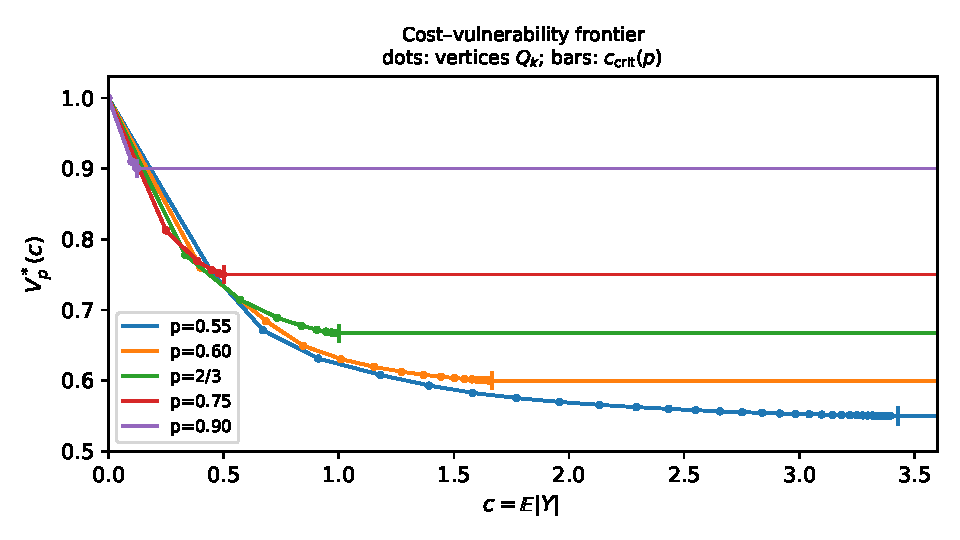
\includegraphics[width=0.85\textwidth]{frontier.pdf}
\caption{Cost--vulnerability frontier for several biases. Dots mark the vertices \(Q_k\); horizontal bars indicate the critical cost \(c_{\mathrm{crit}}(p)\).}
\label{fig:frontier}
\end{figure*}

\begin{figure}[t]
\centering
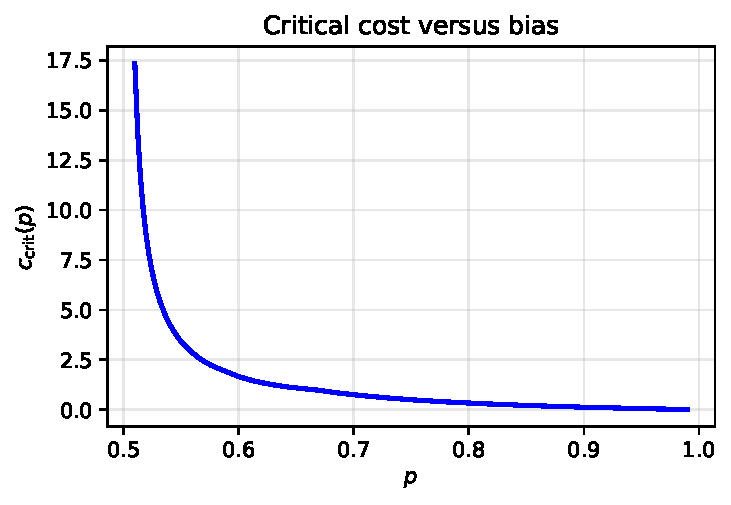
\includegraphics[width=0.9\columnwidth]{ccrit.pdf}
\caption{Critical cost \(c_{\mathrm{crit}}(p)\) as a function of the bias \(p\).}
\label{fig:ccrit}
\end{figure}

\begin{figure}[t]
\centering
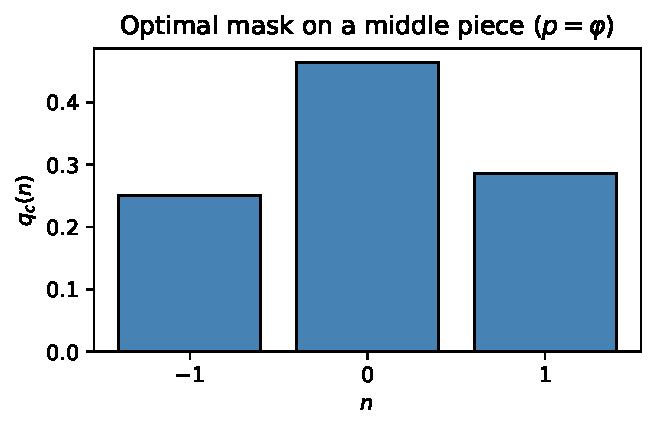
\includegraphics[width=0.9\columnwidth]{optimiser.pdf}
\caption{Example optimal mask on an intermediate piece (\(p=\varphi\approx0.618\), equal mixture of the length-2 and length-3 optimally shifted truncated geometrics). Support is \(\{-1,0,1\}\) with masses approximately \(0.250\), \(0.464\), \(0.286\).}
\label{fig:optimiser}
\end{figure}

\begin{lemma}[Properties of truncated geometrics]\label{lem:T}
(1) \(V_p(T_{L,k})=V_k\) for every \(L\) and every \(k\in\{1,2,\dots,\infty\}\).
(2) The minimal cost of a truncated geometric of length \(k\) is \(C_k\), attained by the shift \(L=-m_k\).
(3) \(m_k\) is nondecreasing in \(k\), increases by at most 1 at each step, and \(m_k\to\ell^*\).
See Appendix~\ref{app:T} for the proof.
\end{lemma}

\begin{lemma}[Convex position]\label{lem:convexpos}
Let \(E_k=(C_{k+1}-C_k)/(u_k-u_{k+1})\). Then \(E_k\) is given by the formula of Theorem~\ref{thm:frontier}, and \(E_1=1-a\). For \(k\ge2\) the increment \(E_k-E_{k-1}\) equals \(1-a^k\) if neither \(k-1\) nor \(k\) is a transition; \((1-\theta_k)(1-a^k)\) if \(k\) is a transition; and \(\bigl(2a^{m_k}-1-a^{k}\bigr)+\theta_{k-1}(1-a^{k-1})\) if \(k-1\) is a transition. In particular \(E_k\) is nondecreasing, \(E_k\ge1-a>0\), and \(E_k\to\infty\). Moreover \(E_k=E_{k-1}\) if and only if \(k\) is a tie.
See Appendix~\ref{app:convex} for the proof.
\end{lemma}

\begin{lemma}\label{lem:limit}
\(C_k\to\ccrit(p)\) and \(V_k\to p\).
\end{lemma}

\begin{proof}[Proof of Theorem~\ref{thm:frontier}]
Let \(g\) be the right-hand side of the theorem, with \(\sigma_k=(V_k-V_{k+1})/(C_{k+1}-C_k)\). Since \(V_k-V_{k+1}=(2p-1)(u_k-u_{k+1})\), we have \(\sigma_k=(2p-1)/E_k\). By Lemma~\ref{lem:convexpos}, \(C_k\) is strictly increasing, and \(\sigma_k\) is positive, nonincreasing and tends to \(0\). With Lemma~\ref{lem:limit}, \(g\) is well defined, continuous, nonincreasing and convex on \([0,\infty)\), since its slopes \(-\sigma_1\le-\sigma_2\le\dots\le0\) are nondecreasing. Also \(g(C_k)=V_k\) and \(g(\ccrit)=p\).

\emph{Lower bound.} Let \(\E_q|N|\le c\), and let \(\nu\) be the measure on truncated geometrics arising from the layer-cake decomposition of \(q\). Set \(C_\infty=\ccrit(p)\) and \(V_\infty=p\). By Lemma~\ref{lem:T} and Theorem~\ref{thm:ccrit}, \(V_p(T_{L,k})=V_k\) and \(\E_{T_{L,k}}|N|\ge C_k\) for all \(k\le\infty\). We use \(g(C_k)=V_k\), then Jensen's inequality for the convex function \(g\), then monotonicity of \(g\):
\begin{align*}
V_p(q)&=\int V_k\,d\nu=\int g(C_k)\,d\nu\\
&\ge g\Bigl(\int C_k\,d\nu\Bigr)\ \ge\ g\bigl(\E_q|N|\bigr)\ \ge\ g(c).
\end{align*}

\emph{Upper bound.} For \(C_k\le c\le C_{k+1}\), the mixture \(q_c\) of Lemma~\ref{lem:T}(2) has cost \(\vartheta C_k+(1-\vartheta)C_{k+1}=c\). By convexity of \(V_p\) and Lemma~\ref{lem:T}(1), \(V_p(q_c)\le\vartheta V_k+(1-\vartheta)V_{k+1}=g(c)\). For \(c\ge\ccrit(p)\), \(G_{-\ell^*}\) is feasible and has \(V_p=p\). Hence \(V_p^*=g\). The statements about the slopes are Lemma~\ref{lem:convexpos}.
\end{proof}

\begin{corollary}[Infinitely many pieces]\label{cor:pieces}
The pieces \([C_k,C_{k+1}]\) are infinitely many and accumulate only at \(\ccrit(p)\). The left derivative at \(\ccrit(p)\) is \(0\). Two adjacent pieces have equal slopes if and only if \(k\) is a tie. There are at most \(\ell^*\) ties.
\end{corollary}

\begin{corollary}[Structure of optimisers]\label{cor:structure}
On each piece the optimiser is a mixture of two adjacent truncated geometrics, with a free residual at exactly one endpoint.
\end{corollary}

\subsection{The first pieces and explicit dual certificates}
\begin{corollary}[Certified cells]\label{cor:cells}
Let \(1/2<p\le\varphi\), \(a=(1-p)/p\), and
\[
c_1=\frac{1+a^2}{1+a+a^2},\qquad c_2=\frac{1+a^2+2a^3}{1+a+a^2+a^3}.
\]
Then \(1-p<c_1<c_2\) and
\[
V_p^*(c)=\begin{cases}
p+\dfrac{(1-p)^2}{p}(1-c), & 1-p\le c\le c_1,\\[2mm]
1-p+p^3(2-c), & c_1\le c\le c_2.
\end{cases}
\]
On the first piece the optimiser is \(q(-1)=c-a(1-c)\), \(q(0)=1-c\), \(q(1)=a(1-c)\). On the second piece, with \(t=p^2(2-c)\), the optimiser is \(q(-1)=t\), \(q(0)=at\), \(q(1)=a^2t\), \(q(2)=1-t(1+a+a^2)\). Both affine functions are lower bounds on \(V_p^*(c)\) for every \(c\ge0\).
\end{corollary}

\section{Design implications}
The explicit frontier supplies concrete design guidance. For a given budget \(c\) and bias \(p\), one simply identifies the unique piece \([C_k,C_{k+1}]\) containing \(c\) and deploys the corresponding mixture of two optimally shifted truncated geometrics. The mixture weights are linear in \(c\), and the free residual mass (which may be placed arbitrarily far away without affecting the objective or the cost to first order) can be used for secondary design goals such as support minimisation or robustness.

Near the critical cost the slope vanishes, so further reductions in vulnerability become arbitrarily expensive. In practice this means that once the budget exceeds roughly \(c_{\mathrm{crit}}(p)\), additional noise yields negligible improvement against a one-guess adversary.

The one-guess vulnerability studied here is operationally distinct from both maximal leakage and mutual information. Maximal leakage equals \(\log\sum_y\max_x\Prob(Y=y\mid X=x)\) and is maximised by a different mechanism under the same absolute-moment budget; mutual information penalises the entire posterior rather than only the single best guess. The exact frontier derived above therefore supplies design guidance that cannot be read off from either of those quantities.

\section{Limitations and future work}
The model is elementary: one observation, one guess, independence, and a pure absolute-moment cost. For the biased bit the frontier has been determined. Several questions remain open. First, uniqueness of the optimiser on intermediate pieces (apart from the degeneracy at ties). Second, priors on three or more points beyond the uniform case. Third, other cost functions, the modular analogue \(Y=X+N\bmod n\), and the case of multiple guesses.

\section{Conclusion}
The optimal additive integer masks have been determined for a uniform interval secret and, for a biased bit, along the entire cost--vulnerability frontier. The results supply exact design guidance for the average one-guess metric under an absolute-moment budget.

\section*{Acknowledgment}
AI tools were used to assist with drafting, proof structuring, figure generation and verification scripts. The author remains fully responsible for the accuracy of all statements, proofs and numerical results.

\bibliographystyle{IEEEtran}
\bibliography{references}

\appendices
\section{Proof of the truncated-geometric properties}
\label{app:T}

\begin{proof}[Proof of Lemma~\ref{lem:T}]
(1) Write \(T=T_{L,k}\). By the excess representation,
\[
V_p(T)=p+\sum_y\max\bigl(0,(1-p)T(y-1)-p\,T(y)\bigr).
\]
On the support \(\{L,\dots,L+k-1\}\) one has \(T(y)=c\,a^{y-L}\) with \(c=(1-a)/(1-a^k)\). The only positive excess occurs at the left endpoint \(y=L\), where the excess mass equals \((1-p)c-p\cdot0=(1-p)c\). All other sites contribute zero excess because the geometric ratio is exactly \(a\). Summing the single excess term yields
\[
V_p(T)=p+(1-p)c=p+(2p-1)u_k=V_k,
\]
independent of \(L\). The pure-geometric case \(k=\infty\) is identical after the optimal shift (the excess vanishes).

(2) The absolute-moment cost of a shift-\(L\) truncated geometric is
\[
\E|T_{L,k}|=\sum_{j=0}^{k-1}|L+j|\,c\,a^j,\qquad c=\frac{1-a}{1-a^k}.
\]
The first difference \(\Delta(L)=\E|T_{L+1,k}|-\E|T_{L,k}|\) equals
\[
\Delta(L)=c\sum_{j=0}^{k-1}\operatorname{sign}(L+j+1/2)\,a^j.
\]
This difference is negative for \(L<-m_k\), zero or positive for \(L\ge-m_k\), and changes sign precisely when the cumulative geometric mass to the left of the origin reaches half the total mass on the truncated support. The integer \(m_k\) is defined exactly as the largest index satisfying that half-mass condition (\(2a^j>1+a^k\)). Substituting \(L=-m_k\) and summing the two finite geometric series (positive and negative parts) produces the closed form
\[
C_k=\frac{a}{1-a}+(m_k-2A_{m_k})+u_k\bigl(2(m_k-A_{m_k})-k\bigr).
\]

(3) If \(k\) increases by one, the half-mass inequality \(2a^j>1+a^k\) can become true for at most one new index \(j\), because the right-hand side decreases by the factor \(a\) while the left-hand side is fixed for each \(j\). Hence \(m_{k+1}\in\{m_k,m_k+1\}\). The sequence is nondecreasing and increases by at most one. It converges to \(\ell^*\) because the pure-geometric median characterised in Theorem~\ref{thm:ccrit} is the pointwise limit of the truncated medians.
\end{proof}

\section{Proof of the convex-position lemma}
\label{app:convex}

\begin{proof}[Proof of Lemma~\ref{lem:convexpos}]
Direct subtraction of the closed forms for \(C_k\) and \(C_{k+1}\) yields
\[
C_{k+1}-C_k=(u_k-u_{k+1})E_k
\]
with the expression for \(E_k\) given in Theorem~\ref{thm:frontier}. For the increments three exhaustive cases arise.

- No transition at \(k-1\) or \(k\): \(m_k=m_{k-1}\) and \(m_{k+1}=m_k\). The difference of the closed forms simplifies to
  \[
  E_k-E_{k-1}=1-a^k\ge0.
  \]
- Transition at \(k\): \(m_{k+1}=m_k+1\). The extra median term contributes a factor \(\theta_k\), and the difference becomes
  \[
  E_k-E_{k-1}=(1-\theta_k)(1-a^k)\ge0.
  \]
- Transition at \(k-1\): the previous step introduced a median, so the difference equals
  \[
  E_k-E_{k-1}=\bigl(2a^{m_k}-1-a^k\bigr)+\theta_{k-1}(1-a^{k-1})\ge0.
  \]

Equality holds in the second or third case precisely when the transition is a tie (\(2a^{m_k+1}=1+a^k\)). Thus \(E_k\) is nondecreasing, \(E_k\ge1-a>0\), and \(E_k\to\infty\). The slope claims follow at once from \(\sigma_k=(2p-1)/E_k\).
\end{proof}

\paragraph{Numerical values of the first points.}
\begin{center}
\begin{tabular}{c|cc|cc}
\(k\) & \(C_k\) (\(p=0.6\)) & \(V_k\) & \(C_k\) (\(p=0.8\)) & \(V_k\) \\
\hline
1 & 0 & 1 & 0 & 1 \\
2 & 0.4 & 0.84 & 0.2 & 0.84 \\
3 & 0.784 & 0.7696 & 0.36 & 0.776 \\
4 & 1.1104 & 0.737 & 0.488 & 0.748 \\
5 & 1.377 & 0.718 & 0.590 & 0.732 \\
\end{tabular}
\end{center}
(The values are exact rational evaluations of the closed forms; rounding is for display.)

\paragraph{Peeling additivity.}
At each stage the residual \(q^{(i)}\) satisfies \(d^{(i)}(n)=q^{(i)}(n)-a\,q^{(i)}(n-1)\ge0\) on the support that remains. The maximal length \(k_i\) is chosen so that the scaled truncated geometric \(\alpha_i T_{L_i,k_i}\) exactly matches the leftmost positive excess layer. Subtracting it removes that layer and leaves a non-negative residual. Because vulnerability is linear in the excesses and the absolute-moment cost is linear, both quantities add exactly across the countable mixture. The process terminates almost surely under the absolute-moment constraint (Markov tightness). The accompanying scripts verify the finite-truncation identities algebraically; the argument above is self-contained for the infinite case.

\end{document}
